    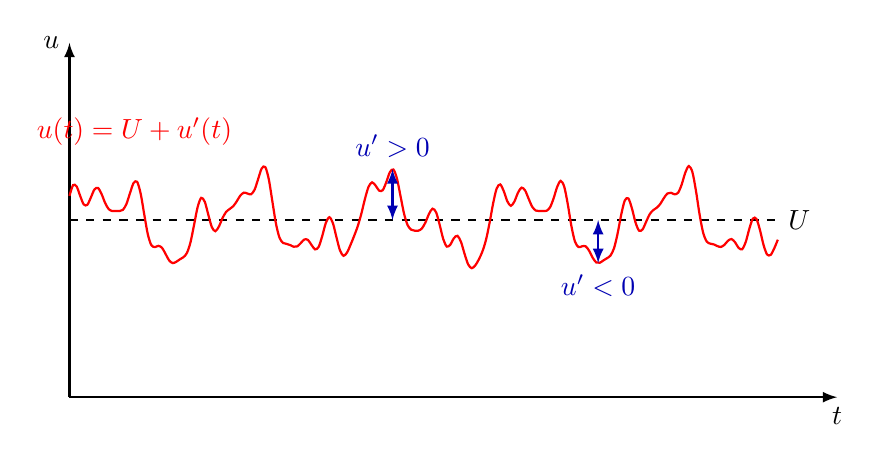
\begin{tikzpicture}[scale=1.5, >=latex]
        % --- SETTINGS ---
        \def\T{6}          % Time duration
        \def\MeanU{1.5}    % Mean velocity height
        \def\Amp{0.5}      % Amplitude of fluctuation
        
        % --- AXES ---
        \draw[->, thick] (0, 0) -- (\T+0.5, 0) node[below] {$t$};
        \draw[->, thick] (0, 0) -- (0, 3.0) node[left] {$u$};
        
        % --- MEAN VELOCITY (U) ---
        \draw[dashed, thick] (0, \MeanU) -- (\T, \MeanU) node[right] {$U$};
        
        % --- INSTANTANEOUS VELOCITY (u = U + u') ---
        % We generate a "random-looking" smooth signal by summing sine waves
        % u(t) = U + sum( A_i * sin(w_i * t + phi_i) )
        \draw[thick, red, smooth, samples=200, domain=0:\T] plot (\x, {
            \MeanU + \Amp * (
                0.5 * sin(300*\x) + 
                0.3 * sin(700*\x + 40) + 
                0.2 * sin(1300*\x + 90) + 
                0.1 * sin(2000*\x + 10)
            )
        });
        
        % --- LABELS: instantaneous u(t) and fluctuation u'(t) = u - U ---
        \node[red, above] at (0.55, 2.05) {$u(t) = U + u'(t)$};
        \draw[<->, thick, blue!70!black] (2.735, \MeanU) -- (2.735, 1.931);
        \node[blue!70!black, above] at (2.735, 1.95) {$u'>0$};
        \draw[<->, thick, blue!70!black] (4.476, \MeanU) -- (4.476, 1.135);
        \node[blue!70!black, below] at (4.476, 1.12) {$u'<0$};
    \end{tikzpicture}
